\section{Interferometry and the actual Inverse Problem} \label{radio}

The simplified inverse Problem says that each antenna pair measures a Fourier Component (Visibility) of the sky. 
\begin{equation}\label{radio:eq:2dft}
V(u, v) = \int\int X(x, y) e^{2 \pi i (ux+vy)} dx dx
\end{equation}

But that is not true, the UV space actually has a third component W. image \ref{radio:uvw} shows it. W is a vector in the direction of the science target.
V is what we measure, X is the image. calculating X is the inverse fourier transform

\begin{figure}[h!] 
	\centering
	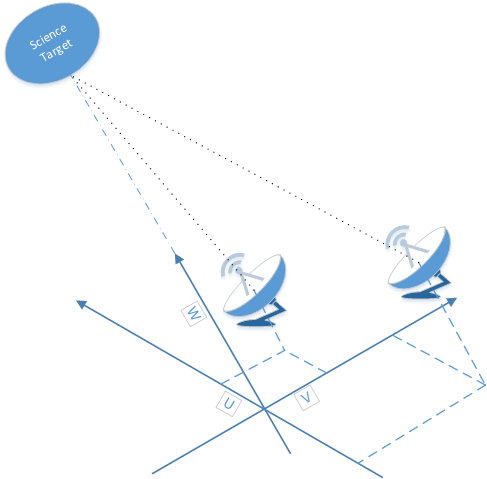
\includegraphics[width=0.6\linewidth]{./chapters/03.radio/uvw.png}
	\caption{U V and W coordinate space}
	\label{radio:uvw}
\end{figure}

\begin{equation}\label{radio:eq:ft}
V(u, v) = \int\int X(x, y) e^{2 \pi i (ux+vy+ w\sqrt{1 - x^2 - y ^2})} \frac{dx dy}{\sqrt{1 - x^2 - y ^2}}
\end{equation}

for small field of view the term  $x^2 + y^2 << 1$ and therefore can be neglected. so we arrive at the 2d fourier transform. for wide field of view, the term.

"The field of view of a telescope is limited by the primary beams of the antennas. To map a region of sky where the emission is at a scale larger than the angular width of the primary beams, mosaicing needs to be done. This is discussed in the second part of this lecture."
Phase 

source : %http://www.gmrt.ncra.tifr.res.in/gmrt_hpage/Users/doc/WEBLF/LFRA/node125.html


\subsection{Calibration}
A lot of effects, weather, noise, antenna temperature, drift.

Antenna based calibration, holds true for current interferometers but is not true for SKA. Possible switch to baseline based calibration